\begin{frame}[fragile]{Tutorial: Two-site circuit optimization}

\begin{columns}

\begin{column}{5cm}

\begin{onlyenv}<1-1>
\begin{lstlisting}[language=JuliaLocal, style=julia, mathescape, basicstyle=\scriptsize\ttfamily]
# Circuit as a vector of gates:
U($\theta$, i1, i2) = [
  op("Ry",i1;$\theta$=$\theta$[1]),
  op("Ry",i2;$\theta$=$\theta$[2]),
  op("CX",i1,i2),
  op("Ry",i1;$\theta$=$\theta$[3]),
  op("Ry",i2;$\theta$=$\theta$[4])]


 \end{lstlisting}
\end{onlyenv}

\begin{onlyenv}<2->
\begin{lstlisting}[language=JuliaLocal, style=julia, mathescape, basicstyle=\scriptsize\ttfamily]
# PastaQ notation:
u($\theta$) = [
  ("Ry",1,(;$\theta$=$\theta$[1])),
  ("Ry",2,(;$\theta$=$\theta$[2])),
  ("CNOT",1,2),
  ("Ry",1,(;$\theta$=$\theta$[3])),
  ("Ry",2,(;$\theta$=$\theta$[4]))]

U($\theta$,i1,i2) =
 buildcircuit(u($\theta$),[i1,i2])
\end{lstlisting}
\end{onlyenv}

\end{column}

\begin{column}{5cm}

\begin{onlyenv}<1->
\vspace*{0.0cm}
\begin{center}
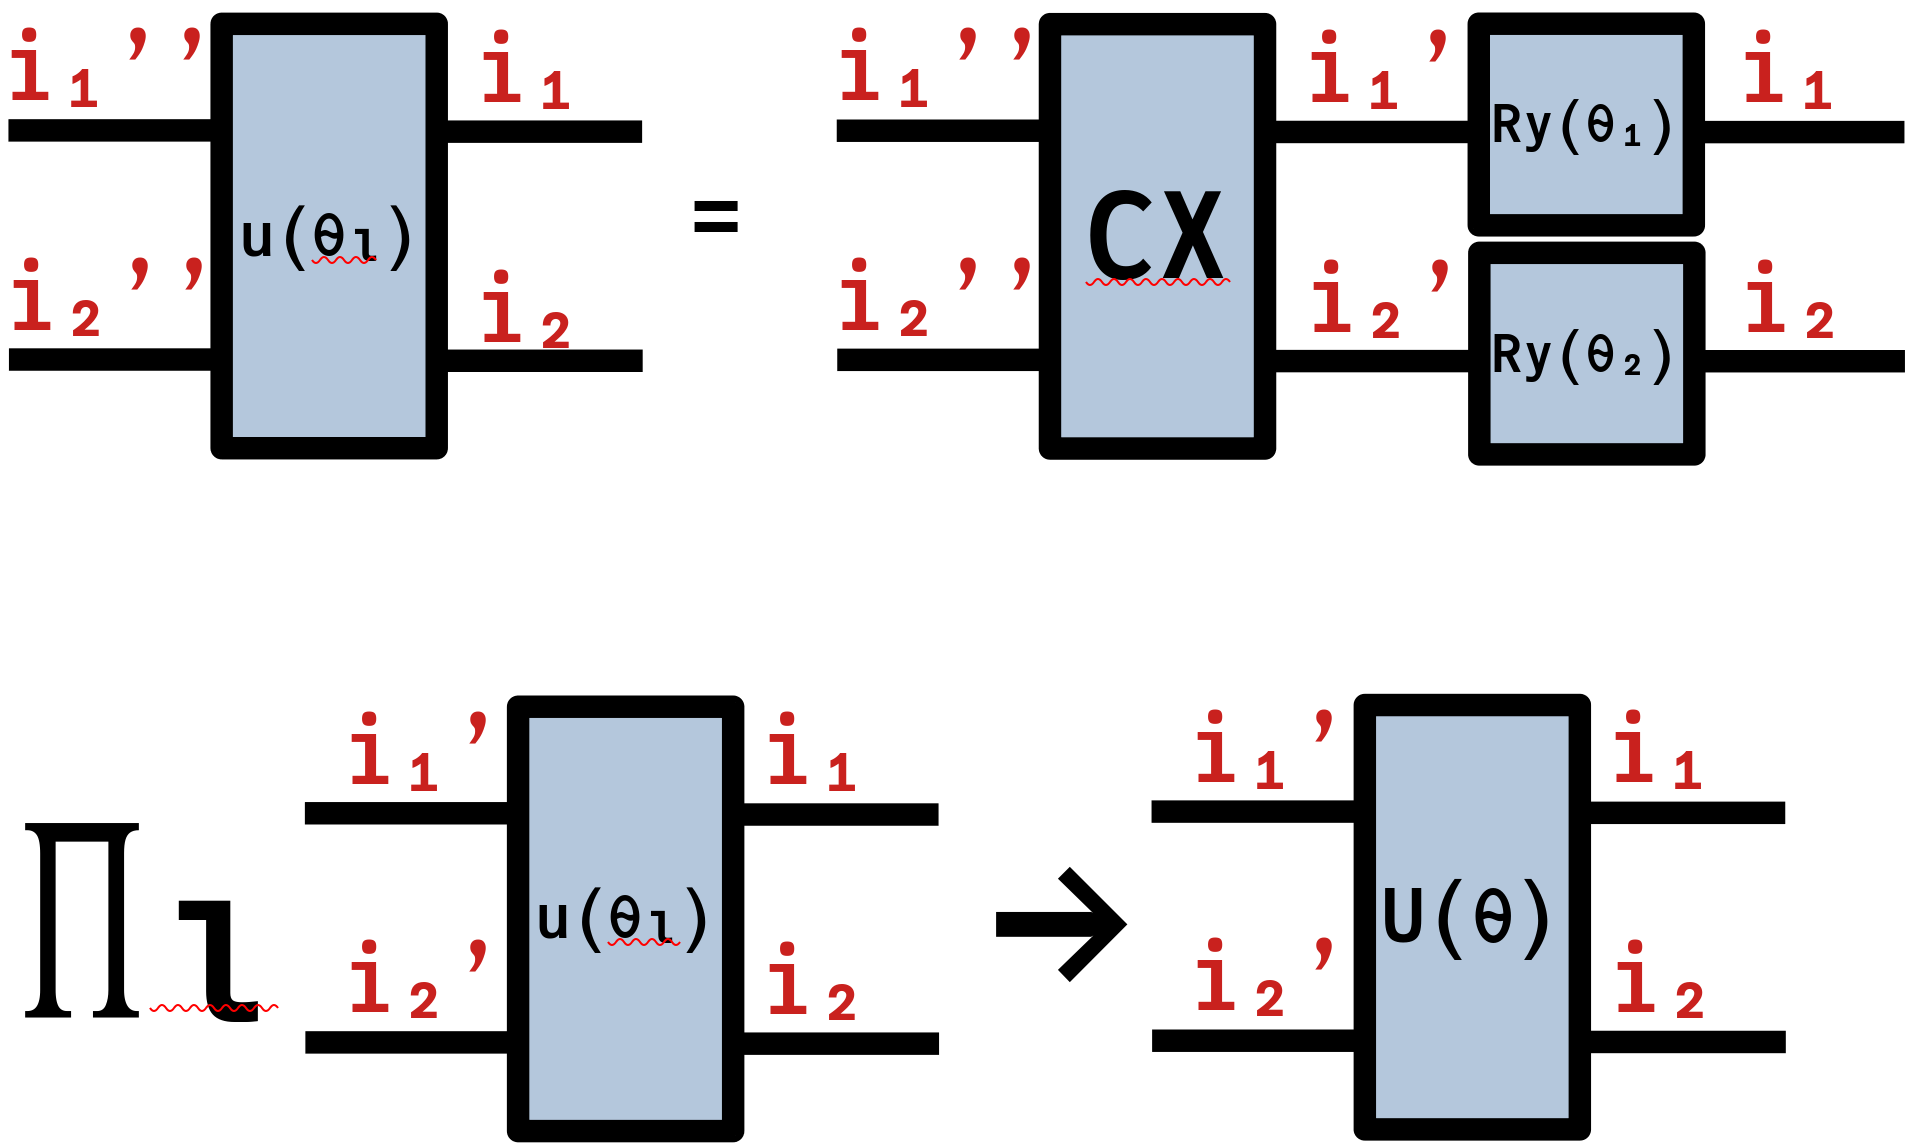
\includegraphics[width=1.0\textwidth]{
  slides/assets/U12.png
}
\end{center}
\vspace*{0.0cm}
\end{onlyenv}

\end{column}

\end{columns}

\end{frame}
